\section{Theory}

The JK flip flop, named after Jack Kilby who invented it is
the most commonly used flip-flop.
It is basically a gated SR flip-flop with the addition of a clock input circuitry that prevents the illegal or invalid output condition that can occur when both inputs $S=R=1$. Due to this additional clocked input, a JK flip-flop has four possible output combinations -- $1$, $0$, \textit{hold} and \textit{toggle}.

\begin{figure}[H]
    \centering
    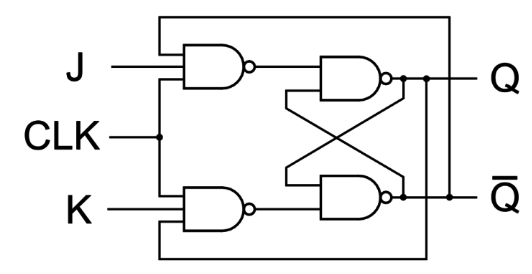
\includegraphics[width=0.65\columnwidth]{images/jk.png}
    \caption{Circuit diagram of a JK flip-flop}
\end{figure}

Assume the clock signal is 1. If $J=1$ and $K=0$, it behaves as a typical SR latch, i.e. $Q=1$ and $Q'=0$. Similarly for $J=0$ and $K=1$, $Q=0$ and $Q'=1$. If both $J=K=0$, then it remains in the same state as it was before i.e. the \verb|HOLD| state.
But if both $J=K=1$, the flip-flop changes state whenever a clock
pulse occurs; i.e., the clock pulse toggles the flip-flop again and again until the Clk goes to 0. This is called is \textbf{race-around condition} (Fig. \ref{race}).

\begin{figure}[H]
    \centering
    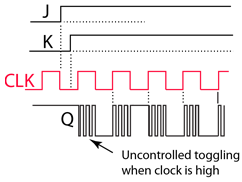
\includegraphics[width=0.5\columnwidth]{images/jkrace.png}
    \caption{Diagram depicting JK racing when the clock is high}
    \label{race}
\end{figure}

To eliminate the race around condition, the following methods can be used:

\begin{itemize}[itemsep=5pt]
    \item \textbf{Increasing the delay of flip-flop}\\
    The propagation delay ($\Delta t$) should be made greater than the duration of the clock pulse (T). But it is not a good solution as increasing the delay will decrease the speed of the system.
    \item \textbf{Use of edge-triggered flip-flop}\\
    If the clock is \verb|HIGH| for a time interval less than the propagation delay of the flip flop then racing around condition can be eliminated. This is done by using the edge-triggered flip flop rather than using the level-triggered flip-flop.
    \item \textbf{Use of master-slave JK flip-flop}\\
    If the flip flop is made to toggle over one clock period then racing around condition can be eliminated. This is done by using Master-Slave JK flip-flop.
\end{itemize}

Now, practically a signal cannot travel instantaneously. Hence any signal will take some finite amount of time to transition between two a lower threshold and an upper threshold. \textbf{Rise time} measures the time taken for the signal to go from 10\% to 90\% of the signal high level. Similarly, \textbf{fall-time} measures the time taken for the signal to go from 90\% to 10\% of the signal high level.

\begin{figure}[H]
    \centering
    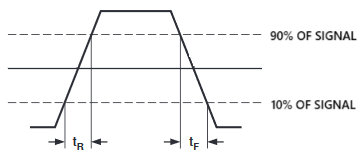
\includegraphics[width=0.75\columnwidth]{images/risediag.png}
    \caption{Rise and fall times depicted in a timing diagram}
\end{figure}

So far we have assumed that at the clock edge, the flip-flop samples the input (or clock signal) and accordingly changes the output immediately. But practically, the flip-flop requires a certain time to respond to the change. Thus any change in the output of the flip flop will occur after a certain delay, also known as the \textbf{propagation delay}.

\begin{figure}[H]
    \centering
    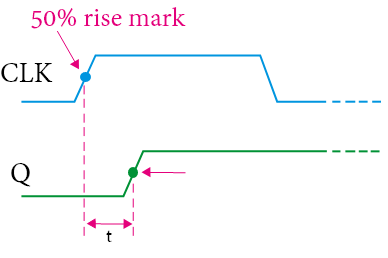
\includegraphics[width=0.7\columnwidth]{images/prop.png}
    \caption{Propagation delay depicted between the clock and Q}
\end{figure}

\section{Apparatus}

\begin{enumerate}
    \item ICs (3 input NAND-7410, NAND-7400)
    \item DC Power Supply (5V)
    \item Oscilloscope
    \item Connecting Wires
    \item Multimeters
    \item Breadboard
\end{enumerate}